\chapter{Introduction}



\section{Autism Spectrum Disorders (ASD)}
Autism is a general term used to describe a spectrum of complex developmental
brain disorders causing qualitative impairments in social interaction and results in
repetitive and stereotyped behaviors. Currently one in every 88 children in the United
States are diagnosed with ASD and government statistics suggest the prevalence rate of
ASD is increasing 10-17 percent annually [9]. Children with ASD experience deficits in
appropriate verbal and nonverbal communication skills including motor control, emotional
facial expressions, and eye gaze attention [10]. Currently, clinical work such as Applied
Behavior Analysis (ABA) [11] [12] has focused on teaching individuals with ASD
appropriate social skills in an effort to make them more successful in social situations [1].
With the concern of the growing number of children diagnosed with ASD, there is a high
demand for finding alternative solutions such as innovative computer technologies and/or
robotics to facilitate autism therapy. Therefore, research into how to design and use modern
technology that would result in clinically robust methodologies for autism intervention is
vital.
In social human interaction, non-verbal facial behaviors (e.g. facial expressions,
gaze direction, and head pose orientation, etc.) convey important information between
individuals. For instance, during an interactive conversation, the peer may regulate their
facial activities and gaze directions actively to indicate the interests or boredom. However,
the majority of individuals with ASD show the lack of exploiting and understanding these
cues to communicate with others. These limiting factors have made crucial difficulties for
individuals with ASD to illustrate their emotions, feelings and also interact with other
human beings. Studies have shown that individuals with autism are much interested to
interact with machines (e.g. computers, iPad, robots, etc.) than humans [6]. In this regard,
in the last decade several studies have been conducted to employ machines in therapy
sessions and examine the behavioral responses of people with autism. These studies have
assisted researchers to better understand, model and improve the social skills of individuals
on the autism spectrum.
This thesis presents the methodology and results of a study that aimed to design a
humanoid-robot therapy sessions for capturing, modeling and enhancing the social skills
of children with Autism. In particular we mainly focus on gaze direction and joint attention
modeling and analysis and investigate how the ASD and Typically Developing (TD)
children employ their gaze for interacting with the robot. In the following section, we have
a brief introduction of the existing assistive robots in the following section and how they
have been used in autism applications.

\section{Socially Assistive Robotics}
Socially Assistive Robotics (SAR) can be considered as the intersection of Assistive
Robotics (AR) and Socially Interactive Robotics (SIR), which has referred to robots that
assist human with physical deficits and also can provide certain terms of social interaction
abilities [5]. SAR contains all properties of SIR described in [6], and also a few additional
attributes such as: 1) user populations (different groups of users, i.e. elders; individuals
with physical impairments; kids diagnosed with ASD; students); 2) social skills (i.e. speech
ability; gestures movement); 3) objective tasks (i.e. tutoring; physical therapy; daily life
assistance); 4) role of the robot (depends on the task the robot has been assigned for) [5].
Companion robots [7] is one type of SAR that are widely used for elderly people
for health care supports. Research shows that this type of social robots can reduce stress
and depression of individuals in elderly stage [8]. Service social robots are able to
accomplish a variety of tasks for individuals with physical impairments [9]. Studies have
shown that SAR can be used in therapy sessions for those individuals who suffer from
cognitive and behavioral disorders (e.g. Autism). SAR provides an efficient helpful
medium to teach certain types of skills to these groups of individuals [10] [11] [12].
Nowadays, there are very few companies that have been designing and producing
socially assistive robots. The majority of existing SARs are not commercialized yet and
because of being expensive and not well-designed user interfaces, they are mostly used forthe research purposes. Honda, Aldebaran Robotics and Hanson Robokind are the top
leading companies that are currently producing humanoid robots.
Ideally socially assistive robots can have fully automated systems to detect and
express social behaviors while interacting with humans. Some of the existing robot-human
interfaces are semi-autonomous and they can recognize some basic biometrics (e.g. visual
and audio commands of the user) and behavioral response. Besides, the majority of existing
robots are very complicated to work with. Therefore in the last couple of years several
companies have started to make these robots more user-friendly and responsive to both the
user need and the potential caregiver commands [5].
Intelligent SARs aim to have the capability to recognize visual or audio commands,
objects, and specific human gestures. Some of these robots have the ability of detect human
face or basic facial expressions. For instance, ASIMO, a robot developed by Honda, it has
a sensor for detecting the movements of multiple objects by using visual information
captured from two cameras on its head. Plus its “eyes” can measure the distance of the
objects from the robot [13]. Another example is from Aldebaran Robotics which designs
small size humanoid robots, called NAO. NAO robot has two cameras attached that are
used to capture single images and video sequences. This capturing module enables NAO
to see the different sides of an object and recognize it for future use. Furthermore, NAO
has a remarkable capability of recognizing faces and detecting moving objects.
Both of the aforementioned robots have speech recognition system. They can interpret
voice commands to accomplish a certain set of tasks which have been pre-programmed in
the system. NAO is able to identify words for running specific commands. However
ASIMO is able to distinguish between voices and other sounds. This feature empowers
ASIMO to perceive the direction of human’s speaker or recognize other companion robots
by tracking their voice [14]. These robots can also speak in many different languages. For
example, NAO can speak in English, French, Chinese, Japanese and other languages up to
more than ten languages. This feature gives the robot a great social communication
functionality to interact with humans from all over the world.

\subsection{Socially Assistive Robots for Autism Therapy}
Socially assistive robots are emerging technologies in the field of robotics that aim
to utilize social robots to increase engagement of users as communicating with robots, and
elicit novel social behaviors through their interaction. One of the goal in SAR is to use
social robots either individually or in conjunction with caregivers to improve social skills
of individuals who have social behavioral deficits. One of the early applications of SAR is
autism rehabilitation. As mentioned before, autism is a spectrum of complex
developmental brain disorders causing qualitative impairments in social interaction.
Children with ASD experience deficits in appropriate verbal and nonverbal communication
skills including motor control, emotional facial expressions, and gaze regulation. These
skill deficits often pose problems in the individual’s ability to establish and maintain social
relationships and may lead to anxiety surrounding social contexts and behaviors [1].
Unfortunately there is no single accepted intervention, treatment, or known cure for
individuals with ASD.
Recent research suggests that children with autism exhibit certain positive social
behaviors when interacting with robots compared to their peers that do not interact with
robots [2][3][4][5][6]. These positive behaviors include showing emotional facial
expressions (e.g., smiling), gesture imitation, and eye gaze attention. Studies show that
these behaviors are rare in children with autism but evidence suggests that robots trigger
children to demonstrate such behaviors. These investigations propose that interaction with
robots may be a promising approach for rehabilitation of children with ASD.
There are several research groups that investigated the response of children with
autism to both humanoid robots and non-humanoid toy-like robots in the hope that these
systems will be useful for understanding affective, communicative, and social differences
seen in individuals with ASD (see Diehl et al., [6]), and to utilize robotic systems to develop
novel interventions and enhance existing treatments for children with ASD [13] [14] [15].
Mazzei et al. [16], for example, designed the robot “FACE” to realistically show the details
of human facial expressions. A combination of hardware, wearable devices, and software
algorithms measured subject’s affective states (e.g., eye gaze attention, facial expressions,vital signals, skin temperature and EDA signals), were used for controlling the robot
reactions and responses.
Reviewing the literature in SAR [5] [6] shows that there are surprisingly very few
studies that used an autonomous robot to model, teach or practice the social skills of
individuals with autism. Amongst, teaching how to regulate eye-gaze attention, perceiving
and expressing emotional facial expressions are the most important ones. Designing robust
interactive games and employing a reliable social robot that can sense users’ socioemotional
behaviors and can respond to emotions through facial expressions or speech is
an interesting area of research. In addition, the therapeutic applications of social robots
impose conditions on the robot’s requirements, feedback model and user interface. In other
words, the robot that aims for autism therapy may not be directly used for depression
treatment and hence every SAR application requires its own attention, research, and
development
Only a few adaptive robot-based interaction settings have been designed and
employed for communication with children with ASD. Proximity-based closed-loop
robotic interaction [29], haptic interaction [30], and adaptive game interactions based on
affective cues inferred from physiological signals [31] are some of these studies. Although
all of these studies were conducted to analyze the functionality of robots for socially interacting with individuals with ASD, these paradigms were limitedly explored and
focused on their core deficits (i.e., Facial expression, eye gaze and joint attention skills).
Bekele and colleagues [32] studied the development and application of a humanoid
robotic system capable of intelligently administering joint attention prompts and adaptively
responding based on within system measurements of gaze and attention. They found out
that preschool children with ASD have more frequent eye contact toward the humanoid
robot agent, and also more accurate respond in joint attention stimulations. This suggests
that robotic systems have the enhancements for successfully improve the coordinated
attention in kids with ASD.
Considering the existing SAR system and the major social deficits that individuals
with autism may have, we have designed and conducted robot-based therapeutic sessions
that are focused on different aspects of social skills of children with autism. In this thesis
we employed NAO which can be remotely controlled to communicate with the children.
We conducted two different protocols to examine the social skills of children with autism
and provide feedbacks to improve their behavioral responses. The contribution of our work
has been introduced in Section 1.4 and the details of the game setting, experiments,
modeling and analysis are provided in Chapter 4.

\section{Music Therapy for ASD}

\section{Thesis Contributions}

\section{Orgizaition}





\subsection{Types of Biometrics} In recent years biometrics moved from simple fingerprinting to many different methods that use
various physical and behavioral measures. The characteristics used
in each category are as follows:

\bi \item Physiological
    \bi
        \item Iris
        \item Fingerprint (including nail)
        \item Hand (including knuckle, palm, vascular)
        \item Face
        \item Retina
        \item DNA
        \item Vein
        \item Ear
        \item Even Odor, Sweat pore, Lips
    \ei
\item Behavioral
    \bi
        \item Signature
        \item Keystroke
        \item Voice
        \item Gait
    \ei
\ei



\bi
\item\textbf{Identification} is a closed-universe (one-to-many) comparing process
for a biometric sample from a given probe against all the known
biometric reference templates in the database. In other words, this
is the answer to the question ``Who am I?'' If the acquired sample
matches a stored template within an acceptable margin of error, then
the identity of the probe is matched to that of the previously
stored reference. During the matching process, a set of similarity
matching scores are obtained for the probe sample (i.e., one-to-many
comparison process). These similarity scores are numerically ranked
such that the highest similarity score is first and the smallest
similarity score is ranked $n$, where $n$ is the number of the
subjects enrolled in the database. In an ideal case, the highest
similarity score is the comparison of the claimed person's biometric
with the same person's biometric that was previously stored in the
database. The percentage of time that the highest similarity score
is the correct match for all individuals, is referred to as the
identification rate.

In order to evaluate the performance of identification, the
percentage of time when one of the top-$r$ matches is correct is
considered and called as ``Cumulative Match score''. In other words,
the ``Cumulative Match Score'' curve is the percentage of correct
identification versus the rank $r$. Usually the percentage of the
correct identification for the rank-one is reported as the
performance of a biometric system.

\item \textbf{Verification} is an open-universe (one-to-one) process of comparing a
submitted biometric sample against single biometric reference of a
single enrollee whose identity or role is being claimed. In other
words, this is the answer to the question, ``Am I who I claim I
am?'' The result of the verification is to confirm that the identity
is matched or not matched. During the process of matching, a
similarity score is computed by the biometric matcher; if the
similarity score is higher than a preset threshold $T$, then the
submitted biometric sample is approved to be the same as the
biometric reference claimed. If the similarity match score is less
than the preset threshold $T$, then the claimed identity for the
submitted biometric is rejected.

In order to evaluate the verification performance, two kinds of
errors can be made by the system: False Match (FM) and False
Non-Match (FNM). FM is the error made by deciding that a (claimed)
identity is a legitimate one while in reality it is an imposter and
FNM is the error made by deciding that a (claimed) identity is not a
legitimate while in reality the person is genuine. The frequency
rate at which FM occurs is called False Match Rate (FMR), and the
frequency rate at which FNM occurs is called False Non-Match Rate
(FNMR). The error rates can be evaluated for any threshold $T$.
Therefore, the functions $FMR(T)$ and $FNMR(T)$ give the error rates
when the match decision is made at threshold $T$. The error rates
can be plotted against each other as a two-dimensional curve,
(FMR(T), FNMR(T)).

This two-dimensional curve is called Receiver Operating
Characteristic (ROC) curve. The ROC curve precisely defines the
complete specification of a biometric matcher and shows the
trade-off between the FMR and FNMR errors over a wide range of
threshold. The biometric matcher can operate using any threshold $T$
which defines a point on the ROC curve. In addition, the ROC can be
used to compare the performance of two biometric matchers against
each other. \ei
\subsection{Biometric Market}
The research service from the Auto ID \& Security business and
financial services group highlights growth sectors of notable
interest and also provides a comprehensive financial analysis of the
biometrics market.  The spotlight on security has intensified
considerably in the wake of global terror attacks and increasing
threats to safety, driving governments across the world to tighten
security measures. The demand for sophisticated security solutions
is greater now than ever before. Figure \ref{fig:anual_revenue}
shows the annual biometric industry revenues for the years 2007-2012
in \$m US. As the Figure shows, the annual revenues in the biometric
market are growing up with a rate of more than 15\% every year. This
is due to the huge demand for the applications of biometric
technology in different fields.

\bfig \epsfig{figure=./chapters/figures/annual_revenue.eps,scale =
0.8} \caption{Annual biometric industry revenues for the years
2007-20012.} \label{fig:anual_revenue}\efig

Figure \ref{fig:percentage_of_biometric_market} shows the percentage
share of the different biometrics in the market in 2006. As the
Figure shows, after Fingerprint (43.6\%), great attention is paid to
face recognition (19.0\%) in the biometric market. Advanced face
recognition biometrics are ideally positioned to address the demand
for security solutions and are set to witness a compound annual
growth rate (CAGR) of 27.5 percent from \$186 million in 2005 to
\$1021.1 million in 2012 \cite{frost06}.

Enhanced credibility of this technology combined with its rapidly
growing awareness is also likely to provide a strong impetus to
growth of the face recognition biometrics market throughout the
forecast period. Concrete evidence in the form of successful
deployments has also helped contribute to continued market growth.

\bfig \epsfig{figure = ./chapters/figures/percent_market.eps, scale
= 0.8} \caption{The percent of biometric market by technology in
2006.} \label{fig:percentage_of_biometric_market}\efig



\btable{\scriptsize \setstretch{1.5}\bt{|c|p{3.5in}|} \hline
\textbf{Category Area} &
\textbf{Applications}\\
\hline

Face ID & Voter registration, Driver licenses, national ID,
immigration \\

\hline

Access Control & Building/room access, computer access \\

\hline

Security & Terrorist alert, secure flight boarding system \\

\hline

Surveillance  &  Advanced video surveillance, nuclear plants
surveillance, neighborhood watch, power grid surveillance, portal control\\

\hline

Smart & Cards stored valued security, user authentication\\

\hline

Law Enforcement & Crime stopping and suspect alert,
shoplifter recognition, suspect background check, post event analysis\\

\hline

Face-based database & Face-based search and retrieval\\

\hline

Multimedia management & Indexing, segmentation, classification, or
event detection \\

\hline

Human computer interaction & Interactive gaming, animation\\
\hline \et} \caption{Typical applications of face.}
\label{tab:face_applications} \etable


\subsubsection{Human Computer Interaction}
Human-computer interaction (HCI) is the study of interaction between
people (users) and computers. To achieve efficient and user-friendly
interaction, the human body part (e.g., the face) could be
considered as a natural input device. For instance the movements of
the face can be used in human tracking system. We recently developed
an efficient tracking system of people based on their facial skin
and body (cloth) colors using a single video camera \cite{Charay05}.
Also, the tracked faces can be used as first step to localize the
location of faces, in video images, for face recognition. Facial
expression recognition is the ability of computers to understand
human emotions. Cohen \etal \cite{Cohen03} reported on several
Advances they have made in building a system for classifying facial
expression from continuous video input. They used Bayesian network
classifiers for classifying expressions from video. Another
application of HCI is realistic synthesis and animation of faces
which are widely used in the video and motion picture industries as
well as the video game industry. Hong \etal \cite{Hong02} designed a
system that provides functionalities for 3-D face modeling and
animation with the help of user interactions. Text and speech
streams can be used to drive the face animation which is used in
computer aided education.

\bi \item Intrinsic variations are independent of any external
sources and are due to the physical nature of the human face.
\item Extrinsic variations are caused by the sources that do not depend on the human
face or any subject under test and are due to the factors such
illumination, viewing geometry, and the imaging process. \ei

Table \ref{tab:variation_face_appearance} summarizes these two types
of variations and their effects on face recognition.

\btable{\scriptsize \setstretch{1.5} \bt{|p{.8in}|p{.7in}|p{3.in}|}
\hline

\textbf{Variation in appearance} & \textbf{Source} & \textbf{Effect/possible task}\\
\hline

Extrinsic & Viewing geometry, Illumination, Imaging process Other
objects & Head Pose light variations, shadow, self shadow
Resolution, scale, focus, sampling Occlusion, shadowing, indirect
illumination, hair, make-up, surgery \\ \hline

Intrinsic & Identity, Facial expression, Age,  Sex,  Speech &
Identification, known-unknown Inference of emotion or intension
Estimating age Decide if male or female Lip reading \\

\hline \et } \caption{Variations in facial appearance Inter-person
and intra-person variations.} \label{tab:variation_face_appearance}
\etable

Among these effects, illumination, variations in pose, aging, and
facial expressions are the most challenging for face recognition.

\bi
\item \textbf{illumination:} Changes in lighting conditions, e.g.,
indoor or outdoor, under which the facial images are captured,
affect the accuracy of face recognition. Variations in illumination
could be caused either by variations in the light source or by
variations in physical parameters of the cameras and the capturing
devices. A solution for this problem is by utilizing the 3-D surface
information of the face. So, by having the 3-D model of the face
surface, the problem reduces to matching the surface geometry of two
faces which are invariant under the effect of illumination.

\item \textbf{Head Pose:} Pose variation is another challenging problem in face
recognition. The variations in pose could be because of the changes
in viewing angle of the camera which causes pose variation in the
2-D or 3-D captured face image. Because face is a 3-D object, 2-D
face recognition under the effect of pose variations is difficult,
while having the 3-D face data, the problem of pose variation can be
handled either in 3-D versus 3-D face recognition or 2-D versus 3-D.

\item\textbf{Facial Expressions:} The development of robust face recognition
algorithm insensitive to facial expression is one of the biggest
challenges of current research in this field. The change in the face
appearance due to its non-rigid structure makes modeling and
analyzing the facial expressions difficult. In addition, facial
expressions vary from person to person, which makes the task of
modeling the facial expressions more difficult.

\item\textbf{Aging Effect:} Aging is the inherent problem of face recognition
because face is an identifier that changes with age and the aging
effect cannot be controlled or ignored. The facial aging effects are
manifested in different forms in different ages. It is manifested as
changes in the shape of the cranium from infancy to teenage while
during the adulthood it is demonstrated as changes in the skin
texture. Thus, because facial aging has different sources, having a
unified solution for this problem is difficult. \ei

Another challenge for face recognition is the need for an evaluation
standard for measuring recognition performance under different
environments and conditions. As a result of this necessity, an
independent government evaluation standard was born, which is
called, Face Recognition Vendor Tests (FRVT). FRVT was developed to
provide evaluations of commercially available and prototype face
recognition technologies. These evaluations are designed to provide
U.S. government and law enforcement agencies with information to
assist them in determining where and how facial recognition
technology can best be deployed. In addition, FRVT results help
identify future research directions for the face recognition
community. In the past, many factors have been evaluated in FRVT
2002 \cite{FRVT2002}. For example, in a verification test with
reasonably controlled lighting, when the gallery consisted of 37,437
individuals with one image per person and the probe set of 74,854
probes with two images per person, the best three systems averaged a
verification rate of 90\% at false accept rate of 1\%, 80\% at false
accept rate of 0.1\%, and 70\% at false accept rate of 0.01\%. This
level of accuracy may be suitable for access control with a small
database of hundreds of people but not for a security system at
airports where the number of passengers is much larger. When
evaluating the performance with respect to pose changes with a
database of 87 individuals, the best system achieved an
identification rate of 42\% for faces within $\pm$45 degrees of
panning and 53\% within $\pm$45 degrees of tilting. Lighting changes
between outdoor probe images and indoor gallery images degrade the
best systems from a verification rate of 90\% to 60\% at a false
accept rate of 1\%.

\section{Proposed Face Modeling and Recognition System}
In Face Recognition Grand Challenge (FRGC) contest, three contenders
for improving face recognition algorithms were considered: high
resolution images, three-dimensional (3-D) face recognition, and
multiple still images. With the 3-D data, the two main challenges of
face recognition, pose variation and illumination, can be handled
easily. This is due to the fact that the 3-D shape of a person's
face is not affected by changes in head orientation and lighting.
Hence, 3-D face recognition has the potential of improving the
recognition performance under these conditions
\cite{3DFaceSurvey2006}. Nevertheless, a pure 3-D face recognition
system has its own following limitations.

\begin{itemize}
\item Capturing the 3-D face data either by a range scanner or by a stereo-based system is slow and expensive
with the current technology.
\item Capturing such a 3-D data is intrusive.
\item Extraction of facial landmarks in 3-D is a very challenging task.
\item Shape matching techniques are complex and time consuming.
\item Lack of the texture cue in captured 3-D range data.
\end{itemize}


\begin{figure}
\begin{center}
\includegraphics[scale = 0.6]{./chapters/figures/3D_ARG_BDG_CH1.eps}\\
\caption{The general block diagram of our system for multi-modal
face recognition based on 3-D ARG
models.}\label{fig_3D_ARG_modeling}
\end{center}
\end{figure}

\begin{figure}
\begin{center}
\includegraphics[scale = 0.5]{./chapters/figures/multi_modal_BDG.eps}\\
\caption{The general block diagram of our system for multi-modal
face recognition based on ridge images and 2-D ARG
models.}\label{fig_gbd_ridge_ARG}
\end{center}
\end{figure}

\begin{figure}
\begin{center}
\includegraphics[scale = 1]{./chapters/figures/3D_performances.eps}\\
\caption{Comparison between the three categories of algorithms for
3-D face recognition, performance of the system versus
complexity.}\label{fig_3-D_comparison}
\end{center}
\end{figure}

\subsubsection{3-D Face Recognition Using 3-D Ridge Images}
In this dissertation, we present a novel method for 3-D face
recognition (shape matching) based on ridge lines extracted from the
3-D range facial images. Compared to other shape matching based
approaches for 3-D face recognition, such as \cite{lu06, russ05,
chang05, Maurer05}, our approach is faster and requires less
computations. This reduction in computations is due to the fact that
we only use the points around the important facial regions on the
face (i.e., the eyes, the nose, and the mouth) and ignore other
surface patches on the face during the matching process. These
points correspond to the extreme ridge points on the considered
surface. An extreme ridge point is a point where the principal
curvature $k_{max}$, has large positive value. There are different
approaches to locate the ridges, here we threshold the $k_{max}$
values to find these points. Figure \ref{fig:ridge_points} shows few
examples of the ridge images obtained by thresholding the $k_{max}$
values. These are 3-D binary images that show the location of the
ridge lines on the surface of the face. In this work, the number of
the points in a ridge image of the face is 12\% $\pm$ 2\% of the
total number of points that cover the face. For matching the ridge
images (probe image versus gallery image), either the Hausdorrf
Distance or the ICP method can be used.

\bfig \epsfig{figure = ./chapters/figures/ridge_image_samples.eps,
scale = 0.8} \caption{Samples of extracted ridge images.}
\label{fig:ridge_points}\efig

\section{Dissertation Contributions}
The major contributions of this dissertation are as follows:
\bi
\item
Improving the Active Shape Model for 2-D facial features extraction
from color image. We present solutions for some of the limitations
of Active Shape Model (ASM) to extract facial feature extraction in
color images.

\item
Developing an algorithm for 3-D facial feature extraction from range
data. Extracting 3-D facial features from 3-D range images is more
difficult compared to 2-D facial feature extraction, because of the
lack of texture in range images. In this dissertation, we develop an
algorithm for extracting three facial feature points (i.e., the
inner corners of the two eyes and the tip of the nose) from facial
range images. These points are used to initially align the ridge
images during the matching process.

\item
Developing an algorithm for 3-D face modeling and recognition based
on ridge images. The ridge lines in the range image carry the most
important distinguishing information of the 3-D face and have high
potential for face recognition. We develop a system for 3-D face
recognition based on ridge lines. For matching the ridge images of
two faces (probe and gallery), the Hausdorff and Iterative Closest
Points are utilized.

\item
Developing a novel algorithm for 3-D face recognition based on
Attributed Relational Graphs (ARG). The nodes of the graph represent
the facial landmark points. A set of attributes are extracted using
Gabor filters and assigned to each node of the graph. Also, a set of
features that defines the mutual relations between the edges of the
graph are extracted and used to increase the performance of the
graph model for face recognition.

\item Developing a multi-modal technique based on the Dempster-Shafer theory
of evidence and the weighted sum rule for fusion at the score level.
\ei

\section{Dissertation Outline}
This thesis is organized as follows: In Chapter two, we present
related work for facial features extraction, two dimensional (2-D),
three dimensional (3-D), and multi-modal (2-D + 3-D) face
recognition. Chapter three explains our algorithm for 2-D facial
feature extraction from frontal face images (i.e., Improved ASM) and
our algorithm for 3-D facial feature extraction (i.e., the
extraction of the three feature points) along with the experimental
results. Chapter four presents our approach for 3-D face modeling
and recognition based on ridge images. Chapter five describes our
multi-modal face modeling and recognition (2-D/3-D) based on
attributed relational graphs along with the experiments. In
addition, we present two fusion techniques for combining the 2-D and
3-D modalities in this chapter. Finally in Chapter six, we present
the conclusion and the future research directions.
